\section{Installing the Board}
The \deviceName\ board can be installed in any PCIe-CEM slot with x1 or more lanes. 
Make sure the PC is powered off and the main power connector is disconnected while installing the board.\par

%
\section{\deviceName\ Inputs and Connectors}
	\subsection{Connectors}
	%
	Figure \ref{fig:schematics} on page \pageref{fig:schematics} shows the location of the inputs on the slot bracket.
%
	\begin{figure*}[hb]
		\begin{center}
			\ifxHPTDC{
				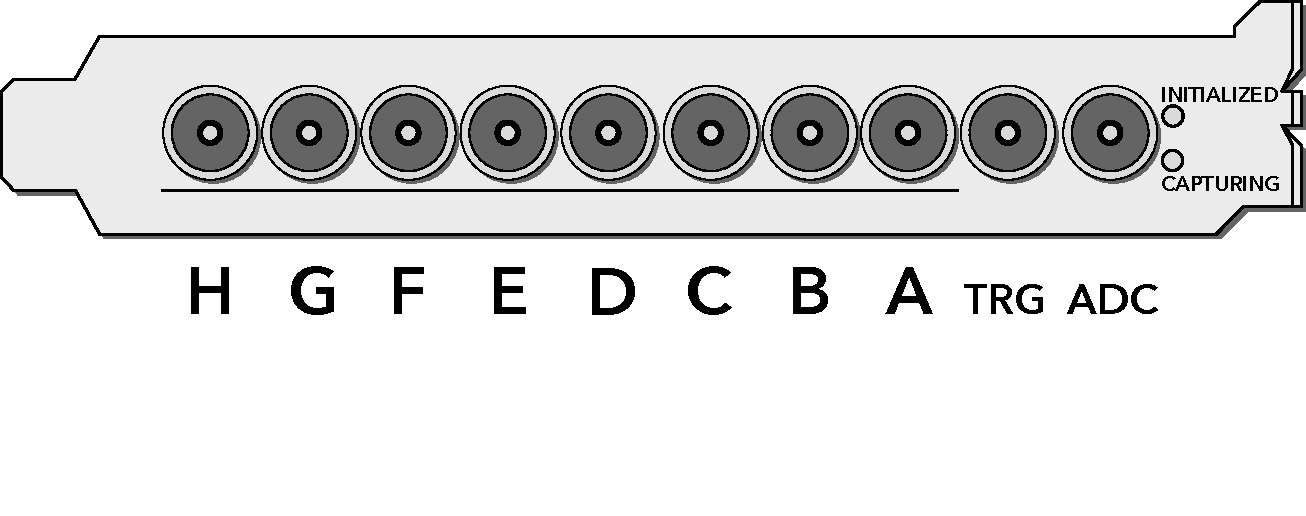
\includegraphics[width=0.6\textwidth]{figures/xHPTDC8_Slotblende.pdf}
			}{
				\includegraphics[width=0.6\textwidth]{figures/xTDC4_Slotblende.pdf}
			}
			\caption{Input connectors of the \deviceName\ on the PCIe bracket.}
		\end{center}
	\end{figure*}
	%
	%
		\begin{figure*}[hb]
			\begin{center}
				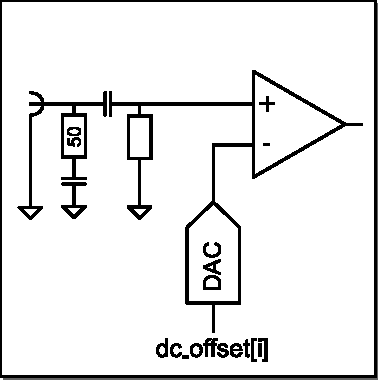
\includegraphics[width=0.3\textwidth]{figures/InputCircuit.pdf}
				\caption{Input circuit for each of the input channels.\label{fig:inputcirc}}
			\end{center}
		\end{figure*}
		%
	Lemo-00 connectors are used for input connection. The inputs are AC-coupled and have an impedance of 50$\Omega$. 
	A schematic of the input circuit is shown in Figure \ref{fig:inputcirc} on page \pageref{fig:inputcirc}. 
	The digital threshold for any input can be adjusted to comply with a manifold of single ended signaling standards.
	The threshold can also be used to configure the input for either positive or negative pulses.
	
	
	The connectors can also be used as outputs. 
	\ifxHPTDC{AC-coupled}{DC-coupled} output pulses for automatic internal triggering and control of external devices 
	can be generated using the TiGer timing pattern generator.

	%
		\begin{figure*}[ht]
			\begin{center}
				\ifxHPTDC{
					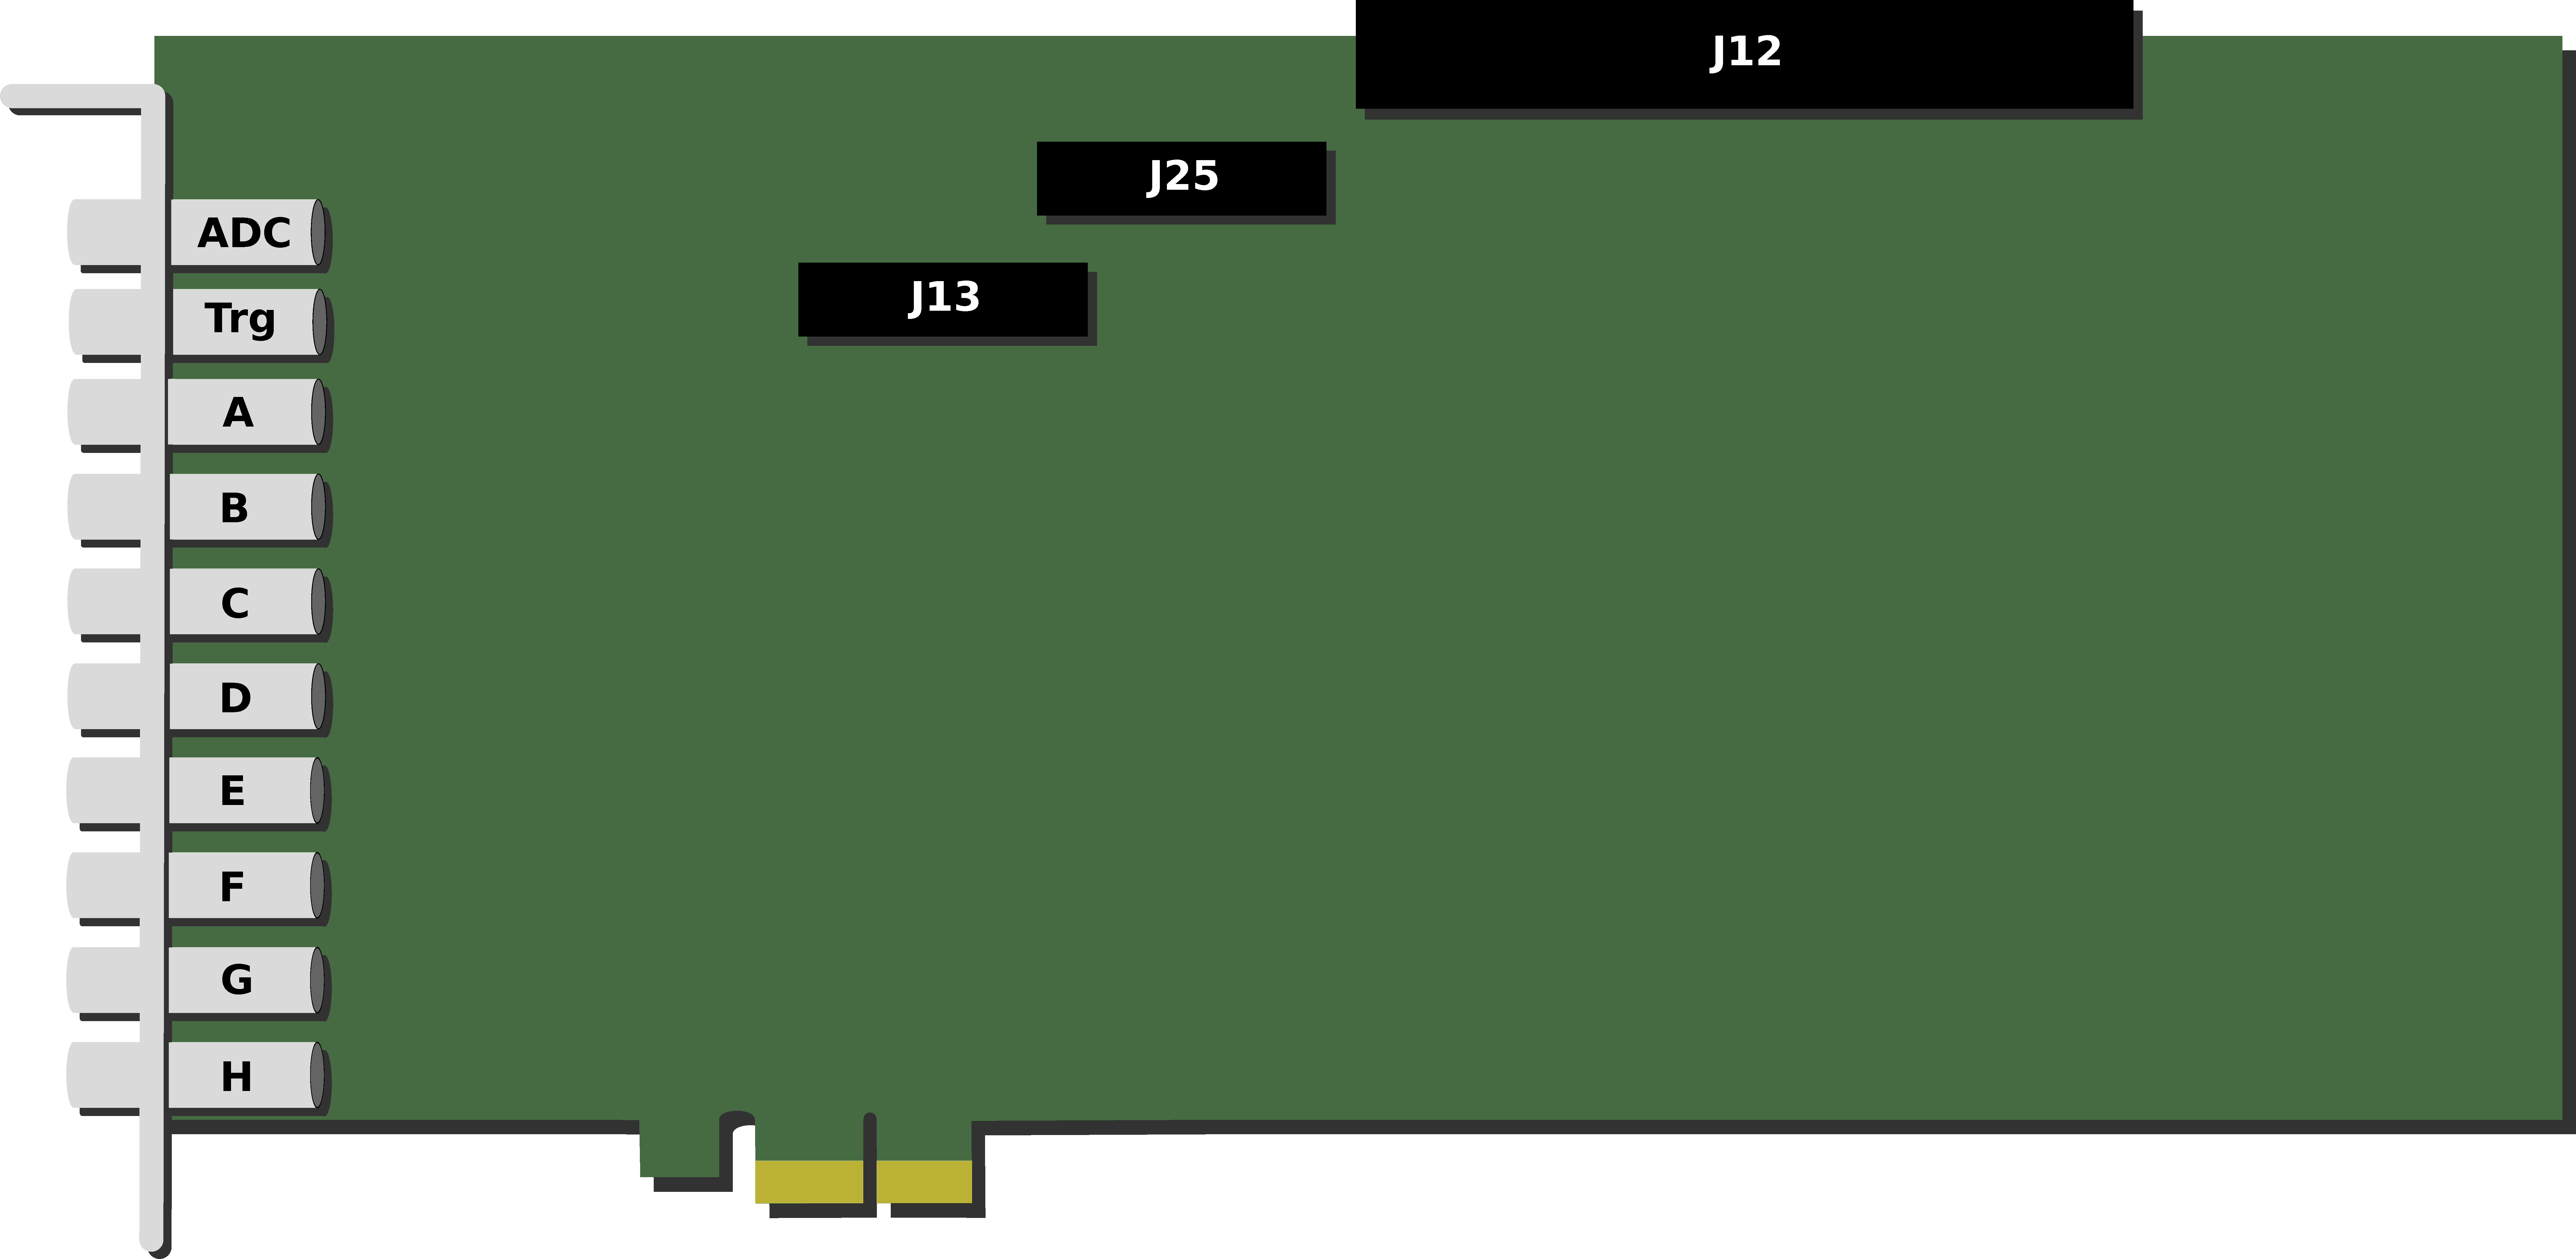
\includegraphics[width=0.7\textwidth]{figures/xHPTDC8_schematic.pdf}
				}{
					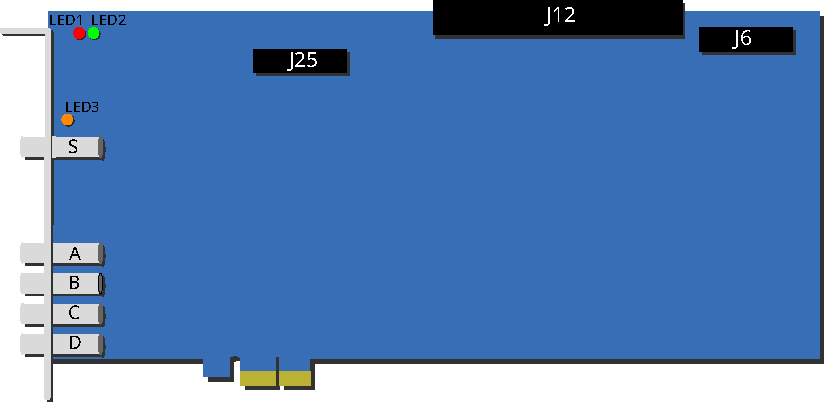
\includegraphics[width=0.7\textwidth]{figures/xTDC4_schematic.pdf}
				}
				
				\caption{Schematic view of a \deviceName\ board showing inter-board connectors C1, C2 and C3.\label{fig:schematics}}
			\end{center}
		\end{figure*}
	%

	Furthermore, three inter board connectors can be found at the top edge of the \deviceName\ board, 
	as displayed in Figure \ref{fig:schematics} on page \pageref{fig:schematics}. 
	Connector J25 is reserved for future use. The pinout of connector J12 is shown in Table \ref{J12} and the pinout of connector J6 is depicted in Table \ref{J6}.

	\begin{table}
	\begin{small}
		\begin{center}
			\begin{tabular}{|c|c|}
				\hline
				Pin & Name\\
				\hline\hline
				1, 2 & GND\\
				\hline
				3, 4 & external CLK in N, external CLK in P\\
				\hline
				5, 6 & GND\\
				\hline
				7, 8 & reserved/NC\\
				\hline
				9, 10 & GND\\
				\hline
				11, 12 & reserved/NC\\
				\hline
				13, 14 & GND\\
				\hline
				15, 16 & reserved/NC\\
				\hline
				17, 18 & GND\\
				\hline
				19, 20 & reserved/NC\\
				\hline
				21, 22 & GND\\
				\hline
				23, 24 & reserved/NC\\
				\hline
				25, 26 & GND\\
				\hline
				27, 28 & reserved/NC\\
				\hline
				29, 30 & GND\\
				\hline
				31, 32 & reserved/NC\\
				\hline
				33, 34 & GND\\
				\hline
			\end{tabular}
			\caption{Pinout of connector J12.}
			\label{J12}
		\end{center}
	\end{small}
	\end{table}

	\begin{table}
	\begin{small}
		\begin{center}
			\begin{tabular}{|c|c|}
				\hline
				Pin & Name\\
				\hline\hline
				1 & +3.3 V\\
				\hline
				2 - 9 & reserved/NC\\
				\hline
				10 & GND\\
				\hline
			\end{tabular}
			\caption{Pinout of connector J6.}
			\label{J6}
		\end{center}
	\end{small}
	\end{table}





	


